\chapter{Informieren}\label{ch:informieren}
Dieses Kapitel zeigt die in der IPERKA-Phase «Informieren» durchgeführten Arbeiten auf. In dieser Phase wird der Einsatzzweck und die Funktionsweise genauer analysiert. Basierend darauf werden Anforderungen an das Projekt definiert.

\section{Projektumfeld}
In diesem Abschnitt wird das Projektumfeld genauer analysiert und unter anderem grafisch dargestellt. Es gilt den groben Ablauf der Aufgabenstellung zu kennen um die Implementation zu vereinfachen.

\subsection{Einsatzzweck}
Momentan sind die Message-Queues nur in der Datenbank ersichtlich. Für den alltäglichen Gebrauch ist das Zugreifen auf die Datenbank umständlich und können Probleme auftreten. Da wenig bis gar keine Sicherheitsmassnahmen bei der Bearbeitung von Elementen in der Datenbank existieren, kann das Unterbrüche und andere Probleme verursachen. Diese Probe-IPA soll das Lesen und Bearbeiten dieser Message-Queues vereinfachen.

\subsection{Funktion}
Die neue Seite Business Daten soll eine Tabelle beinhalten mit den folgenden Spalten.
\begin{itemize}
	\item MODIFIED\_AT: Die letzte Änderung an der Message-QUEUE
	\item MQ\_QUEUE\_ID: Message-Queue-ID
	\item JOB\_KEY: Der dazugehörige JOB
	\item MESSAGE\_SHORT / \_LONG: Die Nachricht
	\item MQ\_IN\_STATUS: Der Verarveitungs-Status
	\item MQ\_IN\_STATUS\_STRING: Das Verarbeitungs-Ergebnis
	\item MQ\_IN\_STATUS\_STRING: Die Anzahl an Verarbeitugsversuche
\end{itemize}

\newpage
Diese Daten werden dann durch ein Get-Request vom Backend geholt. Das Ziel ist, dass die Daten im Frontend nur noch angezeigt werden müssen für die Mindestanforderungen. Im Backend wird durch eine SQL-Query dafür gesorgt, dass nur die oben genannten Spalten au der Datenbank hervorgehlt werden. In der Abbildung 9.1 ist der Ablauf eines solchen GET-Requests ersichtlich.

\begin{figure}[H]
	\begin{center}
		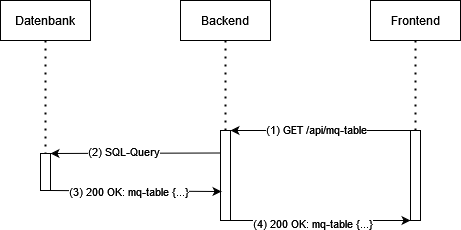
\includegraphics[width=0.8\textwidth]{ressourcen/Ablaufdiagramm}
		\caption[Ablauf eines GET-Requests für das Erstellen der Tabelle]{Ablauf eines GET-Requests für das Erstellen der Tabelle}\label{fig:get-request-for-creation-of-table}
	\end{center}
\end{figure}

Folgende Schritte werden im Ablaufdiagramm durchgeführt.
\begin{enumerate}
	\item Das Frontend sendet einen GET-Request für alle Message-Queues um sie anschliessend in der Tabelle darzustellen.
	\item Das Backend empfängt diesen Request und führt eine SQL-Query aus um die entsprechenden Message-Queues zu erhalten. Die SQL-Query filtert bereits alle Spalten heraus die nicht genutzt werden.
	\item Die Datenbank schickt eine gefilterte Liste mit Message-Queues zurück an das Backend.
	\item Das Backend mappt die entsprechenden Daten in Objekte die das Frontend kennt und schickt es an sie.
\end{enumerate}

Danach kann das Frontend die Daten anzeigen.
\newpage
\section{Anforderungen}
Auf Basis der unter  aufgeführten detaillierten Aufgabestellung und den individuellen Beurteilungskriterien wenden die folgenden Anfortderungen definiert. Die Anforderungen sind den folgenden drei Teilbereichen entsprechend gruppiert und bezeichnet.

\paragraph{MA...} Minimalanforderungen
\paragraph{EP...} Erweiterung Pagination
\paragraph{EF...} Erweiterung Filter

\subsection{Minimalanforderungen}
Folgenden funktionale und nicht funktionale Anforderungen sind hier für die Minimalanforderungen aufgelistet.

\textbf{Funktionale Anforderungen}\newline

\noindent \begin{tabular}{|p{3cm}|p{12cm}|}
	\hline
	\textbf{Anforderung}  & \textbf{Beschreibung} \\ \hline
	MA1    & Die neue Seite ist im Web-GUI auffindbar über den Pfad /admin/mq-table-search und übers Menü unter "Business Daten"→"Queue-Messages".     \\ \hline
	MA2    & Die Tabelle beinhaltet maximal 25 Einträge.     \\ \hline
	MA3    & Alle Einträge sind im Fehlerzustand, d.h. MQ\_IN\_STATUS == 3.     \\ \hline
	MA4    & Die tabellarische Darstellung von MQ\_TABLE beinhaltet volgende Spalten: MODIFIED\_AT, MQ\_QUEUE\_ID, JOB\_KEY, MESSAGE\_SHORT / \_LONG, MQ\_IN\_STATUS, MQ\_IN\_STATUS\_STRING und MQ\_IN\_STATUS\_STRING.    \\ \hline
	MA5    & Anhand von MESSAGE\_IS\_SHORT wird entschieden ob MESSAGE\_SHORT oder MESSAGE\_LONG abgefüllt werden soll.     \\ \hline
	MA6    & Im Web-GUI sollen in der tabellarischen Ansicht nur die ersten 50 Zeichen von MESSAGE\_SHORT / \_LONG angezeigt werde.     \\ \hline
	MA7    & Der MQ\_IN\_STATUS wird in textuelle Stati, gemäss ch.ergon.cardx.shared.database.enumeration.MqInStatus, übersetzt.      \\ \hline
	MA8    & Das Kontextmenü beinhaltet eine Aktion für die Anzeige des kompletten Inhalts der Spalte "Nachricht".     \\ \hline
	MA9    & Das Kontextmenü beinhaltet eine Aktion, um einen erneuten Verarbeitungsversuch eines Eintrages anzustossen. D.h. durch das Setzen des MQ\_IN\_STATUS auf 0.     \\ \hline
	MA10    & Die neuen public-Methoden im Admin-Backend sind mit Unit-Tests bzw. SpringBoot-Tests abgedeckt.Eintrag 4     \\ \hline
	MA11    & Es gibt einen Mock-Datensatz für den neuen MqTable-Rest-Service.     \\ \hline
\end{tabular}

\noindent \textbf{Nicht funktionale Anforderungen}\newline

\noindent \begin{tabular}{|p{3cm}|p{12cm}|}
	\hline
	\textbf{Anforderung}  & \textbf{Beschreibung} \\ \hline
	MA12    & Die Seite ist stimmig ins UI eingebaut, bereits exisiterende UI-Komponenten werden wiederverwendet, oder falls nötig erweitert.     \\ \hline
	MA13    & Die Seite wird in kurzer Zeit geladen, notwendiges Filtering wird auf der Datenbank oder dem Server gemacht.     \\ \hline
\end{tabular}

\subsection{Erweiterung: Pagination}
Folgenden funktionale und nicht funktionale Anforderungen sind hier für die Erweiterung Pagination aufgelistet.

\textbf{Funktionale Anforderungen}\newline

\noindent \begin{tabular}{|p{3cm}|p{12cm}|}
	\hline
	\textbf{Anforderung}  & \textbf{Beschreibung} \\ \hline
	EP1    & Es können mittels Pagination auch mehr als 25 Einträge im Web-GUI angeschaut werden.     \\ \hline
	EP2    & Eine Page beinhaltet maximal 25 Einträge.     \\ \hline
	EP3    & Der Pagination-Mechanismus ist durch Unit-Tests bzw. SpringBoot-Tests abgedeckt.     \\ \hline
\end{tabular} \newline

\noindent \textbf{Nicht funktionale Anforderungen}\newline

\noindent \begin{tabular}{|p{3cm}|p{12cm}|}
	\hline
	\textbf{Anforderung}  & \textbf{Beschreibung} \\ \hline
	EP4    & Einzelne Pages werden erst wenn diese gebraucht werden vom Server geladen.     \\ \hline
	EP5    & Die Navigation zwischen den Seiten ist intuitiv und nutzerfreundlich.     \\ \hline
\end{tabular}

\subsection{Erweiterung: Filter}
Folgenden funktionale und nicht funktionale Anforderungen sind hier für die Erweiterung Filter aufgelistet.

\textbf{Funktionale Anforderungen}\newline

\noindent \begin{tabular}{|p{3cm}|p{12cm}|}
	\hline
	\textbf{Anforderung}  & \textbf{Beschreibung} \\ \hline
	EF1    & Es gibt folgende Filter-Kriterien: Filtern nach MQ\_IN\_STATUS, Filtern mittels Begriffen im Nachrichteninhalt und Filtern nach «Datum von» und «Datum bis»     \\ \hline
	EF2    & Bei Verwendung mehrerer Filter werden diese mittels logischem UND verknüpft.     \\ \hline
	EF3    & Die Filter-Werte können einfach aus dem Web-UI gesetzt werden.     \\ \hline
	EF4    & Die Filterung passiert im Hintergrund, d.h. auf der Datenbank und/oder dem Server.     \\ \hline
	EF5    & Die Einträge sind weiterhin sortiert nach MODIFIED\_DATE.     \\ \hline
	EF6    & Alle Filterkriterien und -werte sind in der URL abgebildet.     \\ \hline
	EF7    & Alle Filter sowie ein Beispiel mit einer Kombination von FIltern sind als Unit-Tests bzw. SpringBoot-Tests abgedeckt.     \\ \hline
\end{tabular}\newline

\newpage
\noindent \textbf{Nicht funktionale Anforderungen}\newline

\noindent \begin{tabular}{|p{3cm}|p{12cm}|}
	\hline
	\textbf{Anforderung}  & \textbf{Beschreibung} \\ \hline
	EF8    & Alle Filterkriterien und -werte sind in der URL abgebildet, um das Speichern und Teilen der Filter zu vereinfachen.     \\ \hline
\end{tabular}

\newpage